% =====================================================================
%  Masamune: A Verdict-Carrying Converter and Plan Language for
%  Chemical Structure Representations
%
%  Self-contained. Every construction is defined here; the paper
%  depends on no companion document.
% =====================================================================
\documentclass[11pt,a4paper]{article}

\usepackage[utf8]{inputenc}
\usepackage[T1]{fontenc}
\usepackage{lmodern}
\usepackage[a4paper,margin=2.4cm]{geometry}
\usepackage{amsmath,amssymb,amsthm,mathtools}
\usepackage{bm}
\usepackage{booktabs}
\usepackage{array}
\usepackage{longtable}
\usepackage{enumitem}
\usepackage{microtype}
\usepackage{xcolor}
\usepackage{listings}
\usepackage{graphicx}
\graphicspath{{figures/}}
\usepackage[round,sort&compress]{natbib}
\usepackage[colorlinks=true,linkcolor=blue!45!black,
            citecolor=blue!45!black,urlcolor=blue!45!black]{hyperref}
\usepackage{cleveref}

% ---- Theorem-like environments ----
\newtheoremstyle{msthm}{\topsep}{\topsep}{\itshape}{}{\bfseries}{.}{.5em}{}
\theoremstyle{msthm}
\newtheorem{theorem}{Theorem}[section]
\newtheorem{lemma}[theorem]{Lemma}
\newtheorem{proposition}[theorem]{Proposition}
\newtheorem{corollary}[theorem]{Corollary}
\theoremstyle{definition}
\newtheorem{definition}[theorem]{Definition}
\newtheorem{rulename}[theorem]{Rule}
\newtheorem{principle}[theorem]{Principle}
\newtheorem{example}[theorem]{Example}
\newtheorem{construction}[theorem]{Construction}
\theoremstyle{remark}
\newtheorem{remark}[theorem]{Remark}
\newtheorem{notation}[theorem]{Notation}

\crefname{rulename}{Rule}{Rules}
\Crefname{rulename}{Rule}{Rules}
\crefname{principle}{Principle}{Principles}
\Crefname{principle}{Principle}{Principles}

% ---- Listing style for masamune plans ----
\definecolor{mskw}{RGB}{30,64,175}
\definecolor{mscom}{RGB}{22,101,52}
\definecolor{msstr}{RGB}{159,18,57}
\definecolor{msns}{RGB}{180,83,9}
\definecolor{msbg}{RGB}{250,250,250}
\lstdefinelanguage{masamune}{
  morekeywords={plan,from,read,translate,require,let,emit,with,as,in,
    when,else,refuse,provenance,budget,source,expect,select,where,
    join,map,via,assert,report},
  morekeywords=[2]{smiles,molfile,sdf,pdb,mmcif,inchi,cml,graph,
    stated,supplied,absent,verdict},
  sensitive=true,
  morecomment=[l]{--},
  morestring=[b]",
  keywordstyle=\color{mskw}\bfseries,
  keywordstyle=[2]\color{msns},
  commentstyle=\color{mscom}\itshape,
  stringstyle=\color{msstr},
  basicstyle=\ttfamily\small,
  backgroundcolor=\color{msbg},
  frame=single,framesep=4pt,xleftmargin=6pt,xrightmargin=4pt,
  breaklines=true,showstringspaces=false,columns=fullflexible,tabsize=2
}
\lstset{language=masamune}

% ---- Shorthand ----
\newcommand{\R}{\mathbb{R}}
\newcommand{\N}{\mathbb{N}}
\newcommand{\Z}{\mathbb{Z}}
\newcommand{\ms}[1]{\texttt{#1}}
\newcommand{\Gph}{\Gamma}
\newcommand{\V}{V}
\newcommand{\E}{E}
\newcommand{\wt}{w}
\newcommand{\med}{\mathsf{m}}
\newcommand{\Prov}{\pi}
\newcommand{\Verd}{\mathsf{v}}
\newcommand{\Src}{\mathsf{S}}
\newcommand{\Feat}{\mathcal{F}}
\newcommand{\Capset}{\mathrm{cap}}
\newcommand{\Req}{\mathrm{req}}
\newcommand{\Ord}{\omega}
\newcommand{\vac}{\nu}
\newcommand{\Capv}{C_v}
\newcommand{\abs}[1]{\lvert#1\rvert}
\newcommand{\bnf}{\;::=\;}
\newcommand{\alt}{\;\mid\;}
\newcommand{\stated}{\textsf{stated}}
\newcommand{\supplied}{\textsf{supplied}}
\newcommand{\absent}{\textsf{absent}}

\title{\textbf{Masamune: A Verdict-Carrying Converter and Plan
Language for Chemical Structure Representations}\\[6pt]
\large Provenance-Typed Translation into Contact Graphs,\\
with Refusal as a First-Class Outcome}

\author{%
Kundai Farai Sachikonye\\
\small Technical University of Munich\\
\small \texttt{kundai.sachikonye@wzw.tum.de}}

\date{\today}

\begin{document}
\maketitle

% =====================================================================
\begin{abstract}
\noindent
A chemical structure arrives at a computation in one of a dozen
formats---a line notation, a connection table, a crystallographic
record---each of which states some things about the molecule and is
silent about others. Converting between them is treated as a solved
engineering problem handled by toolkit calls, and the conversions
themselves are consequently unaudited: a downstream analysis cannot
distinguish a hydrogen the source file recorded from one a valence model
supplied, nor a bond order read from a record from one inferred by a
perception algorithm. We argue that this indistinguishability, not the
conversion difficulty, is the substantive problem, and we specify
\emph{Masamune}, a converter and plan language designed around it.

Masamune translates chemical structure records into \emph{contact
graphs}---finite weighted graphs of atoms, bonds, and a distinguished
\emph{medium} vertex against which every atom is individuated---and it
does so under three disciplines. First, \emph{provenance typing}: every
vertex, every edge, and every attribute carries a tag drawn from
$\{\stated, \supplied, \absent\}$ recording whether the source asserted
it, the converter supplied it from a declared convention, or it is
missing; we prove that provenance is preserved under composition of
conversions (\Cref{thm:prov-compose}) and that the supplied fraction of
a translated graph is computable without re-reading the source
(\Cref{prop:supplied-computable}). Second, \emph{verdict-carrying
translation}: a translation returns a labelled verdict, not a graph
that may or may not be trustworthy, and we prove that a converter
returning a graph-or-nothing interface conflates at least four
distinguishable outcomes which no discipline on its callers can recover
(\Cref{thm:conflation}). Third, \emph{declared capability}: each source
format is characterised by the set of structural features it can state,
and we prove that translation is total and faithful exactly on the
requests whose feature requirements the source's capability set contains
(\Cref{thm:capability}), which makes a large class of translation
failures decidable statically, before any record is read
(\Cref{cor:static}).

On this foundation we build the plan layer. A Masamune plan names
sources, requests records, translates them, and states what it requires
of the result; the plan is checked before execution and refuses, naming
the offending step and feature, when its requirements exceed what its
sources can supply. We give a complete EBNF grammar, a small-step
operational semantics over configurations of store, provenance map and
log, and we prove plan-level determinism and provenance monotonicity
(\Cref{thm:plan-determinism,thm:prov-monotone}).

We report a reference implementation written from this specification and
a translation run over a $48$-structure corpus in two formats. The run
establishes the discipline's practical content: a mean of $73.4\%$ of
the elements of a SMILES-derived contact graph are $\supplied$ rather
than $\stated$, with no structure below $50.0\%$---the majority of a
translated structure is convention, not record. Capability containment
decides $19$ of $24$ format--request pairs before any record is read,
agreeing with the post-read outcome on all $24$. We report four defects
that writing and running the implementation exposed, including a case in
which two faithful representations of the same compound produce contact
graphs that differ while every formula- and identity-level comparison
reports agreement. We state what
Masamune does not do: it does not adjudicate between conflicting
sources, does not repair records, and does not compute chemistry.
\end{abstract}

\noindent\textbf{Keywords:} chemical structure representation; format
conversion; provenance; contact graph; capability calculus; refusal;
plan language; operational semantics; data curation; cheminformatics.

\tableofcontents

% =====================================================================
\part{The Problem}
% =====================================================================

% =====================================================================
\section{Introduction}
\label{sec:intro}
% =====================================================================

\subsection{Six formats, one molecule, six different things said}

Consider ethanol as it appears in six places.

A SMILES string \citep{weininger1988smiles,opensmiles} writes it
\ms{CCO}: three heavy atoms, two bonds, and nothing else. The six
hydrogens are not in the string. They are recoverable, but only by
applying a valence model that the string does not contain and does not
name.

A molfile \citep{dalby1992ctfile} writes an atom block and a bond block.
Depending on how it was produced, the hydrogens may be present as atom
records with coordinates, or absent and implied, or present for some
atoms and absent for others. The file does not say which convention was
used.

A PDB record \citep{berman2000pdb} writes atoms with coordinates and,
usually, no bond block at all: connectivity for standard residues is
supplied from a template library keyed on residue name, and for
non-standard residues from \ms{CONECT} records that may or may not be
present and may or may not be complete.

An mmCIF record \citep{westbrook2022pdbx} writes the same structure with
an explicit chemical component dictionary reference, so connectivity is
stated by reference rather than inferred---but the reference must be
resolved against an external dictionary that the file does not carry.

An InChI string \citep{heller2015inchi} writes a canonical layered
identifier in which the hydrogen layer is explicit but the bond orders
are not: InChI deliberately normalises away the distinction between
tautomers and between certain bond-order assignments, so information
present in the molfile is absent by design.

A CML document \citep{murrayrust2011cml} can state all of the above, or
any subset, because the schema is permissive about which elements are
required.

Each of these is a correct record of ethanol. They differ in what they
\emph{state}. A computation that consumes all six and treats them as
interchangeable inputs is not consuming the same information six times;
it is consuming six different information sets and discarding the
difference.

\subsection{The problem is not conversion; it is what conversion hides}

Conversion between these formats is well-trodden ground. Mature
toolkits---RDKit \citep{rdkit}, Open Babel \citep{oboyle2011openbabel},
the CDK \citep{willighagen2017cdk}---read and write all of them
competently, and the algorithmic difficulties (ring perception,
aromaticity models, stereochemistry) are documented and largely solved
in the sense that reasonable implementations agree most of the time.

What is not solved, and what this paper is about, is that \emph{the
output of a conversion does not record what the conversion did}. When a
toolkit reads \ms{CCO} and produces a molecule object with nine atoms,
the six added hydrogens are indistinguishable, in the object and in
everything downstream of it, from six hydrogens that had been written in
the file. When a PDB reader assigns bond orders from a residue template,
the resulting double bond is indistinguishable from one that was stated
in a \ms{CONECT}-bearing record. When an aromaticity perceiver marks a
ring aromatic, the resulting bond kind is indistinguishable from an
aromatic bond written by the depositor.

This matters for three reasons that are not cosmetic.

\paragraph{Errors become unattributable.} Structure errors in public
collections are common and well documented
\citep{young2008errors,fourches2010curation,williams2012quality,%
akhondi2012consistency}, and a substantial fraction arise not from
mis-drawn structures but from conversions that supplied something the
source did not state. Without provenance the two are indistinguishable
at the point of use, so a downstream anomaly cannot be traced to the
step that introduced it.

\paragraph{Agreement becomes uninformative.} Two pipelines that agree on
a result may agree because both read the same stated facts, or because
both applied the same convention to the same silence. These are
epistemically different situations and the second is much weaker
evidence, but a result set that does not carry provenance cannot
distinguish them.

\paragraph{Absence becomes invisible.} A format that cannot state a
feature and a record that declines to state it produce the same output:
nothing. The distinction between \emph{this source cannot say} and
\emph{this record does not say} is exactly the distinction a curator
needs and exactly the one that is lost.

\subsection{What Masamune is}

Masamune is a converter from chemical structure records to \emph{contact
graphs}, and a plan language for expressing federated queries whose
results are contact graphs. It is designed so that the three
indistinguishabilities above are impossible to produce.

The target representation is fixed and simple: a finite weighted graph
whose vertices are atoms plus a distinguished \emph{medium} vertex
representing everything the molecule is individuated against, whose
edges are contacts, and whose weights are separation costs
(\Cref{sec:graph}). We choose this target because it is the weakest
structure that supports the operations chemical computations actually
perform---separating a part from the rest, comparing what two structures
hold in common---and because every claim in this paper is then a claim
about a finite weighted graph, checkable by anyone who grants only that
such graphs exist.

The three disciplines are:

\begin{enumerate}[label=(D\arabic*),leftmargin=3em,itemsep=3pt]
\item \textbf{Provenance typing} (\Cref{sec:provenance}). Every element
of a translated graph carries a tag in $\{\stated,\supplied,\absent\}$.
The tags compose (\Cref{thm:prov-compose}), so a chain of conversions
reports its own reliability, and the supplied fraction is computable
from the graph alone (\Cref{prop:supplied-computable}).

\item \textbf{Verdict-carrying translation} (\Cref{sec:verdicts}). A
translation returns a labelled verdict with a payload, and a graph
appears only under the label that warrants it. We prove that the
conventional interface---return a molecule, signal failure by returning
nothing---conflates four distinguishable outcomes, and that the
conflation is a property of the interface rather than of its use
(\Cref{thm:conflation}).

\item \textbf{Declared capability} (\Cref{sec:capability}). A source
format is characterised by the features it can state. Translation is
total and faithful exactly on requests contained in that set
(\Cref{thm:capability}), and containment is decidable before any record
is read (\Cref{cor:static}).
\end{enumerate}

The plan layer (\Cref{sec:plans}) makes these usable at scale: a plan
declares its sources and its requirements, is checked statically, and
refuses with a named cause rather than producing a result whose
trustworthiness the caller must guess.

\subsection{What Masamune is not}

Three exclusions are stated here and repeated with their consequences in
\Cref{sec:limits}.

Masamune does not \emph{adjudicate}. When two sources disagree about a
structure, Masamune reports two graphs with their provenances and the
locus of disagreement; it does not decide which is right. Adjudication
requires chemistry Masamune does not have.

Masamune does not \emph{repair}. A record that cannot be translated
faithfully produces a refusal naming the obstruction, not a best-effort
graph. Repair is a curation decision belonging to a person
\citep{fourches2016curation2}.

Masamune does not \emph{compute chemistry}. It produces contact graphs;
what is computed on them is outside this specification. The claims here
are about faithfulness of translation and about what the resulting
object records, never about chemical correctness of the source.

\subsection{Contributions}

\begin{enumerate}[label=(\roman*),leftmargin=2.2em,itemsep=2pt]
\item A target representation for chemical structure---the contact
graph---defined in full, with the medium vertex made explicit rather
than left implicit in a solvent model (\Cref{sec:graph}).
\item A provenance calculus over translations, with composition and
computability results (\Cref{sec:provenance}).
\item A six-valued verdict algebra and a proof that the conventional
converter interface cannot represent it (\Cref{sec:verdicts}).
\item A capability calculus deciding translatability statically
(\Cref{sec:capability}).
\item A plan language with grammar, operational semantics, and
determinism and monotonicity theorems (\Cref{sec:plans,sec:semantics}).
\item A reference implementation, a $48$-structure run across two
formats, and four specification defects found by implementing and
running it (\Cref{sec:implementation}).
\end{enumerate}

% =====================================================================
\section{Related work and what is new}
\label{sec:related}
% =====================================================================

\paragraph{Format conversion.} The toolkits
\citep{rdkit,oboyle2011openbabel,willighagen2017cdk} solve the
conversion problem in the sense of producing correct structures from
correct inputs, and their internal models are richer than the contact
graph we target. What they do not provide is a record, surviving into
the output, of which parts of the structure came from the input. Our
contribution is not a better reader but a typed output.

\paragraph{Canonicalisation.} InChI \citep{heller2015inchi} and
canonical SMILES \citep{weininger1989smiles2,oboyle2012inchi} address a
different problem: assigning a unique string to a structure so that
identity comparison is string comparison. Canonicalisation deliberately
normalises away distinctions (tautomers, certain bond-order
assignments), which is correct for identity and lossy for provenance.
SELFIES \citep{krenn2020selfies} guarantees syntactic validity of
generated strings, again a different goal. A canonical form answers
``are these the same structure''; Masamune answers ``what did each
source actually say''.

\paragraph{Curation.} The curation literature
\citep{fourches2010curation,fourches2016curation2,williams2012quality,%
young2008errors} establishes both that structure errors are prevalent
and that systematic protocols reduce them. Those protocols are
procedures for humans and scripts to follow. Masamune's contribution is
to make one part of such a protocol---knowing what was supplied---a
property of the data structure rather than of the discipline with which
a procedure was followed.

\paragraph{Provenance in databases.} Why-, how-, and where-provenance
\citep{buneman2001why,cheney2009provenance} and the PROV model
\citep{moreau2013prov} formalise the tracking of derivation through
query evaluation. Our provenance is coarser and specialised: three tags
on structural elements rather than a derivation history. The
specialisation buys a composition law with a closed form
(\Cref{thm:prov-compose}) and a per-graph statistic computable in one
pass (\Cref{prop:supplied-computable}).

\paragraph{Nulls and missing information.} That an empty result and a
failure are different, and that conflating them corrupts downstream
reasoning, is the null-value problem
\citep{codd1979extending,imielinski1984incomplete,libkin2016sql} in a
new setting. \Cref{sec:verdicts} is a six-valued refinement specific to
structure translation, and \Cref{thm:conflation} is the corresponding
inexpressibility result.

\paragraph{Capability-aware querying.} Query planning over sources with
restricted answering ability is classical, and query-language expressive
power is well characterised
\citep{perez2009sparql,angles2017foundations}. Our capability calculus
(\Cref{sec:capability}) is in that lineage; the difference is that a
capability shortfall yields a typed verdict the plan can route around
rather than a planning failure.

\paragraph{Workflow systems.} Workflow engines
\citep{koster2012snakemake,ditommaso2017nextflow} supply control flow
over file-producing steps and are widely used to run conversion
pipelines. They do not know what a step means, so a conversion executed
inside a workflow node is as unaudited as one executed in a script.
Masamune's plan layer is narrower and typed: its steps are translations,
and their verdicts are part of the language.

% =====================================================================
\part{The Target}
% =====================================================================

% =====================================================================
\section{The contact graph}
\label{sec:graph}
% =====================================================================

We fix the object every translation produces.

\subsection{Definition}

\begin{definition}[Contact graph]
\label{def:contact}
A \emph{contact graph} is a tuple $\Gph=(\V,\E,\wt,\med)$ where $\V$ is
a finite non-empty vertex set, $\E\subseteq\binom{\V}{2}$ is a set of
unordered pairs, $\wt\colon\E\to\R_{>0}$ assigns each pair a strictly
positive \emph{contact weight}, and $\med\in\V$ is a distinguished
vertex, the \emph{medium}, with $\{v,\med\}\in\E$ for every
$v\in\V\setminus\{\med\}$. Vertices other than $\med$ are \emph{items};
an edge between two items is a \emph{contact}. We write
$\Omega=\sum_{e\in\E}\wt(e)$ for the total weight.
\end{definition}

Three points about this definition are load-bearing.

\emph{The medium is explicit.} Most molecular representations leave the
environment implicit: a molfile records a molecule, not a molecule in a
solvent. Making $\med$ a vertex forces a translation to say what each
atom is individuated \emph{against}, which is where the difference
between a buried atom and an exposed one lives. No claim about what the
medium physically is enters any result below; it is a structural slot.

\emph{Weights are separation costs, not distances.} $\wt(\{u,v\})$ is
read as the cost of telling $u$ from $v$, and such costs add along a
cut, whereas distances do not. This is why the target is a weighted
graph rather than an embedding.

\emph{Positivity is required.} $\wt>0$ everywhere. A zero-weight edge
would assert that two items are separable at no cost, i.e.\ are not
distinct; the representation excludes this by construction.

\begin{definition}[Cut and separation cost]
\label{def:cut}
For $S\subseteq\V$ the \emph{cut} is
$\partial(S)=\{\{u,v\}\in\E: \abs{\{u,v\}\cap S}=1\}$ with weight
$\wt(\partial(S))=\sum_{e\in\partial(S)}\wt(e)$. For an item $v$ the
\emph{separation cost} is
\begin{equation}
\sigma(v)\;=\;\min_{S\ni v,\ \med\notin S}\wt(\partial(S)),
\label{eq:sepcost}
\end{equation}
the minimum weight of a cut placing $v$ on one side and the medium on
the other. The minimum is over a finite non-empty family, hence attained,
and equals a maximum flow \citep{fordfulkerson1956}, computable exactly
\citep{stoer1997simple,gomory1961multi}.
\end{definition}

\begin{lemma}[Separation costs are positive]
\label{lem:positive}
For every item $v$, $\sigma(v)>0$.
\end{lemma}

\begin{proof}
Any admissible $S$ contains $v$ and omits $\med$, and $\{v,\med\}\in\E$
by \Cref{def:contact}, so $\{v,\med\}\in\partial(S)$ and hence
$\partial(S)\ne\varnothing$. Since $\wt>0$ on every edge, every
admissible cut has positive weight, and so does their minimum.
\end{proof}

\Cref{lem:positive} is the reason the medium is required to be adjacent
to everything: it guarantees the separation cost is a well-posed
positive quantity for every item, in every translated graph, without any
assumption about the chemistry.

\subsection{What a translation must produce}

\begin{definition}[Translation target]
\label{def:target}
A \emph{translated structure} is a pair $(\Gph,\Prov)$ where $\Gph$ is a
contact graph and $\Prov$ is a provenance map (\Cref{def:prov}). The
vertex set is $\V=A\cup\{\med\}$ with $A$ the atoms of the structure;
each $a\in A$ carries the attributes of \Cref{def:attrs}; each contact
carries the attributes of \Cref{def:bondattrs}.
\end{definition}

\begin{definition}[Atom attributes]
\label{def:attrs}
An atom vertex carries: the element (equivalently the atomic number
$Z\in\N^{+}$); the formal charge $q\in\Z$; the isotope mass number, or a
marker for unspecified; the count of attached hydrogens; the valence
capacity $\Capv$ and occupancy of its outer shell, from which the
\emph{vacancy} $\vac=\Capv-q_v$; and, when the source supplies them,
Cartesian coordinates.
\end{definition}

\begin{definition}[Contact attributes]
\label{def:bondattrs}
A contact between two atoms carries: the \emph{committed cell count}
$c\in\{1,2,3\}$ for single, double and triple interfaces; a
\emph{delocalised} marker for contacts belonging to a delocalised system,
which carries the system's identity rather than an integer count; and,
when the source supplies it, stereochemical configuration.
\end{definition}

\begin{remark}[Why cell count rather than bond order alone]
\label{rem:cellcount}
The committed cell count records how many valence cells the interface
commits, which is the quantity a separation must sever. For an ordinary
double bond this coincides with the bond order. It is separated from
bond order in name because a delocalised system commits cells that
belong to no single pairwise interface, and forcing such a system into a
per-bond integer---the familiar $1.5$---asserts a pairwise fact the
source did not state. \Cref{def:bondattrs} therefore carries
delocalisation as a marker over a set of contacts, and
\Cref{prop:deloc} records what follows.
\end{remark}

\begin{proposition}[Delocalisation is not a per-bond attribute]
\label{prop:deloc}
Let $R$ be a set of contacts marked as one delocalised system. There is
in general no assignment of committed cell counts to the individual
contacts of $R$ that both sums to the system's total committed cells and
is determined by the source record. Consequently a representation
assigning each contact of $R$ a numeric count states something the
source did not.
\end{proposition}

\begin{proof}
Take $R$ a six-membered delocalised ring committing nine cells in total
(six $\sigma$, three delocalised). Any per-bond assignment
$(c_1,\dots,c_6)$ with $\sum_i c_i=9$ and $c_i\in\{1,2\}$ requires
exactly three $c_i=2$, and there are two such assignments related by
rotation---the two Kekul\'e forms. Both satisfy the total. The source, if
it stated only that the ring is delocalised, does not distinguish them;
selecting one is therefore an assertion not present in the record. If
instead fractional counts $c_i=1.5$ are assigned, the assignment states
that each pairwise interface commits one and a half cells, which is a
pairwise claim, whereas the source's claim was about the ring.
\end{proof}

\Cref{prop:deloc} is why \Cref{def:bondattrs} has a marker and not a
number, and it is the first place where the provenance discipline of the
next section is forced rather than chosen: the alternative is to state
something and tag it $\supplied$, which is admissible but must be
visible.

% =====================================================================
\part{The Three Disciplines}
% =====================================================================

% =====================================================================
\section{Provenance typing}
\label{sec:provenance}
% =====================================================================

\subsection{The three tags}

\begin{definition}[Provenance tags]
\label{def:tags}
The provenance tag set is $P=\{\stated,\supplied,\absent\}$ with the
readings: $\stated$---the source record asserts this element;
$\supplied$---the converter produced this element by applying a declared
convention to the source's silence; $\absent$---neither the source nor
any applicable convention determines this element, and it is missing
from the graph.
\end{definition}

\begin{definition}[Provenance map]
\label{def:prov}
A \emph{provenance map} for a translated structure is a function
$\Prov$ assigning a tag in $P$ to each vertex, each edge, and each
attribute of each vertex and edge. We write $\Prov(x)$ for the tag of
element $x$.
\end{definition}

\begin{notation}[Conventions]
\label{not:conventions}
A \emph{convention} is a named, documented rule for supplying an element
the source does not state---for example, ``implicit hydrogens are
supplied to fill the standard valence of each organic-subset atom''
\citep{opensmiles}. Every $\supplied$ element carries the name of the
convention that produced it, so that $\Prov$ is not merely a tag but an
attribution.
\end{notation}

\begin{principle}[No silent supply]
\label{prin:nosilent}
A converter may supply any element for which it has a declared
convention. It may not supply an element without tagging it $\supplied$
and naming the convention. An element that is neither stated nor
supplied is $\absent$ and is not present in the graph.
\end{principle}

\Cref{prin:nosilent} is the whole discipline, and everything in this
section is a consequence of enforcing it.

\begin{example}[Ethanol from three sources]
\label{ex:ethanol}
From \ms{CCO}: three atom vertices $\stated$; two contacts $\stated$
with cell count $1$ $\stated$; six hydrogen vertices $\supplied$ by the
organic-subset valence convention, with their contacts $\supplied$; all
coordinates $\absent$.

From a molfile with explicit hydrogens and coordinates: nine atom
vertices $\stated$; eight contacts $\stated$; all coordinates $\stated$.

From a PDB record with no \ms{CONECT} lines: nine atom vertices
$\stated$ with coordinates $\stated$; contacts $\supplied$ by whichever
connectivity convention the converter declares---template lookup or
distance-based perception---and cell counts $\supplied$ or $\absent$
depending on the convention.

The three graphs have the same vertex and edge sets. They have
different provenance maps, and that difference is the information the
conventional pipeline discards.
\end{example}

\subsection{Composition}

Conversions compose: a record may be read in one format, written in
another, and read again. We need to know what happens to provenance.

\begin{definition}[Composition of tags]
\label{def:compose}
Define $\oplus\colon P\times P\to P$ by
\[
\begin{array}{c|ccc}
\oplus & \stated & \supplied & \absent\\\hline
\stated & \stated & \supplied & \absent\\
\supplied & \supplied & \supplied & \absent\\
\absent & \absent & \absent & \absent
\end{array}
\]
read as: the tag of an element after a second conversion, given its tag
before ($\text{row}$) and the tag the second conversion would assign
($\text{column}$).
\end{definition}

\begin{lemma}[$\oplus$ is associative with absorbing element]
\label{lem:monoid}
$(P,\oplus)$ is a commutative monoid with identity $\stated$ and
absorbing element $\absent$, and $\supplied$ satisfies
$\supplied\oplus\supplied=\supplied$.
\end{lemma}

\begin{proof}
Direct from the table. $\stated$ acts as identity by inspection of the
first row and column. $\absent$ absorbs by inspection of the last row
and column. Commutativity is symmetry of the table. Associativity
follows since $P$ ordered by $\stated<\supplied<\absent$ makes $\oplus$
the binary maximum, which is associative.
\end{proof}

\begin{theorem}[Provenance composes]
\label{thm:prov-compose}
Let $T_1$ and $T_2$ be translations with provenance maps $\Prov_1$ and
$\Prov_2$, and let $T_2\circ T_1$ be their composition. Then for every
element $x$ of the composite output,
\[
\Prov_{T_2\circ T_1}(x)\;=\;\Prov_1(x)\oplus\Prov_2(x),
\]
and consequently: an element is $\stated$ in the composite only if it
was $\stated$ at every stage; an element $\supplied$ at any stage is
$\supplied$ or worse in the composite; and $\absent$ at any stage is
$\absent$ in the composite.
\end{theorem}

\begin{proof}
By \Cref{lem:monoid}, $\oplus$ is the maximum under
$\stated<\supplied<\absent$. It therefore suffices to check the three
clauses. \emph{Stated.} If any stage supplied the element, that stage's
tag is $\supplied$, and the maximum is at least $\supplied$; hence
$\stated$ in the composite requires $\stated$ at every stage.
\emph{Supplied.} If some stage tagged $\supplied$ and no stage tagged
$\absent$, the maximum is $\supplied$. \emph{Absent.} If any stage
tagged $\absent$ the element is not present after that stage, so it is
absent thereafter and the maximum is $\absent$. Associativity
(\Cref{lem:monoid}) extends this from two stages to any finite chain.
\end{proof}

\begin{corollary}[Round-tripping degrades provenance monotonically]
\label{cor:roundtrip}
Writing a translated structure to a format and reading it back cannot
raise any element's provenance. In particular, a structure whose
hydrogens were $\supplied$ and which is written to a format storing
hydrogens explicitly yields, on re-reading, hydrogens tagged
$\stated$ by the second reader and $\supplied$ in the composite.
\end{corollary}

\begin{proof}
Immediate from \Cref{thm:prov-compose}: the composite tag is the
maximum, and the maximum of $\supplied$ with anything other than
$\absent$ is $\supplied$.
\end{proof}

\begin{remark}[Why \Cref{cor:roundtrip} is the point]
\label{rem:roundtrip-why}
Round-tripping is how supplied information conventionally becomes
indistinguishable from stated information: a toolkit adds hydrogens,
writes an SD file, and the next reader sees explicit hydrogen records
with no indication of their origin. \Cref{thm:prov-compose} is precisely
the rule that prevents this, and \Cref{cor:roundtrip} is the guarantee
it buys. Note that it requires provenance to travel \emph{with} the
structure; a format that cannot carry provenance breaks the chain, which
is why \Cref{sec:capability} treats provenance-carrying as a capability
like any other.
\end{remark}

\subsection{The supplied fraction}

\begin{definition}[Supplied fraction]
\label{def:suppfrac}
For a translated structure $(\Gph,\Prov)$ let $X$ be the set of vertices
and edges of $\Gph$. The \emph{supplied fraction} is
\[
\phi(\Gph,\Prov)\;=\;\frac{\abs{\{x\in X : \Prov(x)=\supplied\}}}
{\abs{X}}\;\in\;[0,1].
\]
\end{definition}

\begin{proposition}[The supplied fraction is computable from the graph
alone]
\label{prop:supplied-computable}
$\phi(\Gph,\Prov)$ is computable in time $O(\abs{\V}+\abs{\E})$ from
$(\Gph,\Prov)$, without access to the source record.
\end{proposition}

\begin{proof}
One pass over the vertices and edges reads each element's tag from
$\Prov$ and increments two counters. No clause of \Cref{def:suppfrac}
refers to the source.
\end{proof}

\Cref{prop:supplied-computable} is modest as a theorem and consequential
in practice: it means every downstream consumer can report how much of
its input was convention, at negligible cost, with no cooperation from
the producer beyond carrying $\Prov$.

\begin{remark}[What the supplied fraction does not measure]
\label{rem:suppfrac-limits}
$\phi$ counts elements, not importance. A structure whose single
$\supplied$ element is a bond order at a reactive centre and one whose
twenty $\supplied$ elements are aliphatic hydrogens may have very
different $\phi$ and the opposite ordering of trustworthiness for a
given purpose. $\phi$ is an audit statistic, not a quality score, and
\Cref{sec:limits} records the consequence.
\end{remark}

% =====================================================================
\section{Verdict-carrying translation}
\label{sec:verdicts}
% =====================================================================

\subsection{The six verdicts}

\begin{definition}[Verdict]
\label{def:verdict}
A \emph{verdict} is a pair $\Verd=(\ell,\pi)$ with label $\ell$ drawn
from
\[
L=\{\textsf{translated},\ \textsf{incomplete},\
\textsf{unsupported},\ \textsf{malformed},\
\textsf{underdetermined},\ \textsf{empty}\}
\]
and a label-specific payload $\pi$:
\begin{center}
\small
\begin{tabular}{@{}ll@{}}
\toprule
Label & Payload\\
\midrule
\textsf{translated} & the pair $(\Gph,\Prov)$ and the supplied fraction $\phi$\\
\textsf{incomplete} & the partial element set and the features found $\absent$\\
\textsf{unsupported} & the requested features the source format cannot state\\
\textsf{malformed} & the parse position and the token or record at fault\\
\textsf{underdetermined} & the element admitting several readings, and the readings\\
\textsf{empty} & the source location, certified to contain no structure\\
\bottomrule
\end{tabular}
\end{center}
\end{definition}

\begin{definition}[Assignment]
\label{def:assign}
Given a source record $r$ from format $\Src$ and a request with feature
requirement $\Req$, the verdict is computed by the first applicable
clause:
\begin{enumerate}[label=(V\arabic*),leftmargin=*]
\item if $r$ does not parse under $\Src$'s grammar, return
$(\textsf{malformed},\cdot)$;
\item else if $r$ parses to no structural content, return
$(\textsf{empty},\cdot)$;
\item else if $\Req\not\subseteq\Capset(\Src)$, return
$(\textsf{unsupported},\Req\setminus\Capset(\Src))$;
\item else if some element admits two or more readings under the
declared conventions with no rule selecting between them, return
$(\textsf{underdetermined},\cdot)$;
\item else if some requested element is neither stated nor suppliable,
return $(\textsf{incomplete},\cdot)$;
\item else return $(\textsf{translated},(\Gph,\Prov,\phi))$.
\end{enumerate}
\end{definition}

The clause order is not arbitrary: each clause precedes every clause
whose evidence it would corrupt. (V1) precedes all others because an
unparsed record supports no claim about its content; (V3) precedes (V4)
and (V5) so that a limitation of the \emph{format} is never reported as
a defect of the \emph{record}; and (V4) precedes (V5) because an element
with several readings is not missing.

\begin{proposition}[Only one verdict carries a graph]
\label{prop:one-graph}
Of the six labels, only $\textsf{translated}$ has a payload containing a
contact graph. Consequently the presence of a graph in a verdict
determines $\ell=\textsf{translated}$, and the five other outcomes are
distinguishable from it and from each other by label alone.
\end{proposition}

\begin{proof}
By inspection of the payload table in \Cref{def:verdict}. The
\textsf{incomplete} payload carries an element set, not a graph, and is
explicitly not a contact graph in the sense of \Cref{def:contact}: it
need not satisfy the medium-adjacency condition.
\end{proof}

\begin{remark}[Why \textsf{incomplete} must not carry a partial graph]
\label{rem:no-partial}
It is tempting to have \textsf{incomplete} return whatever was
successfully translated, so a caller can proceed on the part that
worked. This defeats \Cref{prop:one-graph}: a caller receiving a graph
would then have to inspect the label to know whether it is complete,
which is exactly the discipline-on-callers that \Cref{thm:conflation}
below shows cannot be relied upon. A caller that genuinely wants partial
results requests them, by weakening $\Req$ so that clause (V5) does not
fire---which makes the weakening visible in the plan rather than
implicit in the caller's handling.
\end{remark}

\subsection{The conventional interface cannot express this}

\begin{definition}[Graph-or-nothing interface]
\label{def:gon}
A \emph{graph-or-nothing} interface is a function from source records to
$G\cup\{\bot\}$, where $G$ is the set of contact graphs and $\bot$
signals failure, with no channel other than the returned value.
\end{definition}

\begin{theorem}[Four-way conflation]
\label{thm:conflation}
Let $I$ be a graph-or-nothing interface. There exist four source
records, one for each of the labels \textsf{unsupported},
\textsf{malformed}, \textsf{underdetermined} and \textsf{empty}, on
which $I$ returns the same value $\bot$. No property of a caller of $I$
distinguishes them.
\end{theorem}

\begin{proof}
Construct the four records. \emph{Unsupported}: a request for bond
orders against a coordinate-only record; the interface has no graph
satisfying the request, so returns $\bot$. \emph{Malformed}: a record
with a syntax error; no parse, so no graph, so $\bot$.
\emph{Underdetermined}: a record whose delocalised system admits two
readings by \Cref{prop:deloc} with no selecting rule; the interface
cannot return a graph without asserting one reading, so returns $\bot$.
\emph{Empty}: a well-formed record containing no atoms; there is no
contact graph, since \Cref{def:contact} requires a non-empty vertex set,
so $\bot$.

In all four cases the returned value is $\bot$, and these are equal as
values. A caller's subsequent behaviour is a function of the value it
receives; equal values induce equal behaviour. Hence no caller
distinguishes the four, and no discipline imposed on callers changes the
values returned. The conflation is therefore a property of $I$.
\end{proof}

\begin{corollary}[The repair is a wider return type, not better error
handling]
\label{cor:wider}
No wrapper, logging convention, or exception discipline applied to a
graph-or-nothing interface recovers the four-way distinction, since by
\Cref{thm:conflation} the information is absent from the returned value.
Recovering it requires the interface itself to return a verdict.
\end{corollary}

\begin{proof}
A wrapper is a function of $I$'s output; by \Cref{thm:conflation} that
output is constant across the four cases, and a function of a constant
is constant.
\end{proof}

\begin{remark}[Scope of \Cref{thm:conflation}]
\label{rem:conflation-scope}
The theorem does not say existing toolkits are badly engineered; several
do expose diagnostic channels alongside their return values, and a
careful caller can consult them. It says that the \emph{contract} of
returning a structure with failure signalled by its absence has
insufficient capacity, so any recovery depends on out-of-band
information that nothing requires the caller to consult. Making the
verdict the return value makes consultation unavoidable.
\end{remark}

\subsection{An empty result is a result}

\begin{proposition}[Certified emptiness]
\label{prop:certified-empty}
A verdict $(\textsf{empty},\ell)$ is a positive claim: the source
location parsed successfully and contains no structural content. It is
therefore not interchangeable with $(\textsf{malformed},\cdot)$, which
asserts nothing about content, nor with
$(\textsf{unsupported},\cdot)$, which asserts nothing about the record.
\end{proposition}

\begin{proof}
By clause order in \Cref{def:assign}: (V2) is reached only when (V1) did
not fire, so the record parsed; and it fires only when the parse yielded
no structural content. Both facts are therefore established when the
label is emitted, and neither is established by (V1) or (V3).
\end{proof}

% =====================================================================
\section{Declared capability}
\label{sec:capability}
% =====================================================================

\subsection{Features and capability sets}

\begin{definition}[Feature alphabet]
\label{def:features}
The feature alphabet is the finite set
\[
\Feat=\left\{
\begin{array}{l}
\textsf{element},\ \textsf{connectivity},\ \textsf{cellcount},\
\textsf{delocalisation},\\
\textsf{charge},\ \textsf{isotope},\ \textsf{hcount},\
\textsf{stereo},\\
\textsf{coords3d},\ \textsf{conformer},\ \textsf{provenance}
\end{array}
\right\}
\]
where \textsf{element} is the atomic identity of each atom;
\textsf{connectivity} the atom--atom incidence; \textsf{cellcount} the
committed cell count of a contact; \textsf{delocalisation} the marking
of a delocalised system; \textsf{charge} formal charge; \textsf{isotope}
mass number; \textsf{hcount} explicit hydrogen counts;
\textsf{stereo} stereochemical configuration; \textsf{coords3d}
Cartesian coordinates; \textsf{conformer} multiple coordinate sets for
one connectivity; and \textsf{provenance} the ability of the format to
carry a provenance map.
\end{definition}

\begin{definition}[Source and capability set]
\label{def:source}
A \emph{source} is a pair $\Src=(\text{grammar},\Capset(\Src))$ where the
grammar decides parsing and $\Capset(\Src)\subseteq\Feat$ is the
\emph{declared capability set}: the features the format can state.
\end{definition}

\begin{example}[Capability sets of common formats]
\label{ex:caps}
\leavevmode
\begin{center}
\small
\begin{tabular}{@{}lp{0.62\textwidth}@{}}
\toprule
Format & $\Capset$\\
\midrule
SMILES & \textsf{element}, \textsf{connectivity}, \textsf{cellcount},
\textsf{delocalisation}, \textsf{charge}, \textsf{isotope},
\textsf{hcount}, \textsf{stereo}\\
Molfile V2000 & \textsf{element}, \textsf{connectivity},
\textsf{cellcount}, \textsf{charge}, \textsf{isotope}, \textsf{stereo},
\textsf{coords3d}\\
SD file & the molfile set, plus \textsf{conformer} and
\textsf{provenance} (via data fields)\\
PDB & \textsf{element}, \textsf{charge}, \textsf{coords3d},
\textsf{conformer}; \textsf{connectivity} only where \ms{CONECT} is
present\\
mmCIF & \textsf{element}, \textsf{connectivity}, \textsf{cellcount},
\textsf{charge}, \textsf{coords3d}, \textsf{conformer},
\textsf{provenance}\\
InChI & \textsf{element}, \textsf{connectivity}, \textsf{charge},
\textsf{isotope}, \textsf{hcount}, \textsf{stereo}\\
\bottomrule
\end{tabular}
\end{center}
Two entries deserve comment. Molfile V2000 lacks
\textsf{delocalisation} because the aromatic bond type is not part of
the V2000 specification for structures as opposed to queries
\citep{dalby1992ctfile}; a file using it is using a query feature in a
structure record. InChI lacks \textsf{cellcount} by design: the
identifier normalises bond orders away
\citep{heller2015inchi}, which is correct for its purpose and means it
cannot state what a molfile states.
\end{example}

\begin{remark}[A capability set is a claim about a reader, not a
specification]
\label{rem:cap-claim}
$\Capset(\Src)$ as used by an implementation describes what \emph{that
implementation's reader} can faithfully extract from that format, which
may be narrower than what the format specification permits. Declaring
narrowly is safe: it causes some requests to be refused that could have
been served, and never produces a graph asserting something the source
did not state. Declaring broadly is unsound and silent: the reader
claims a feature, produces a graph, and the graph is wrong in a way the
verdict does not reveal. \Cref{sec:limits} records that no mechanical
check enforces honest declaration.
\end{remark}

\subsection{The containment theorem}

\begin{definition}[Faithful translation]
\label{def:faithful}
A translation of record $r$ from $\Src$ is \emph{faithful} if every
element of the resulting graph tagged $\stated$ is asserted by $r$, and
every element asserted by $r$ that lies within the request is present in
the graph.
\end{definition}

\begin{definition}[Honest declaration]
\label{def:honest}
$\Capset(\Src)$ is \emph{honest} if for every $f\in\Feat$: $f\in\Capset(\Src)$
exactly when the reader for $\Src$ extracts $f$ faithfully from every
record of $\Src$ stating it.
\end{definition}

\begin{theorem}[Translation is total and faithful exactly on contained
requests]
\label{thm:capability}
Let $\Src$ have an honest declaration and let $r$ be a record parsing
under $\Src$'s grammar with non-empty content. Then for a request with
feature requirement $\Req$:
\[
\text{the verdict is }\textsf{translated}\text{ or }\textsf{incomplete}
\quad\Longleftrightarrow\quad \Req\subseteq\Capset(\Src),
\]
and when $\Req\not\subseteq\Capset(\Src)$ the verdict is
$(\textsf{unsupported},\Req\setminus\Capset(\Src))$, which by
\Cref{prop:one-graph} carries no graph.
\end{theorem}

\begin{proof}
($\Leftarrow$) Suppose $\Req\subseteq\Capset(\Src)$. Clauses (V1) and (V2)
do not fire by hypothesis. Clause (V3) does not fire since the
containment holds. The verdict is therefore determined by (V4), (V5) or
(V6), which yield \textsf{underdetermined}, \textsf{incomplete} or
\textsf{translated}. Of these, \textsf{underdetermined} arises only when
a declared convention fails to select among readings, which is a
property of the conventions rather than of containment; excluding that
case, the verdict is \textsf{translated} or \textsf{incomplete}, and by
honesty (\Cref{def:honest}) every feature of $\Req$ that $r$ states is
extracted faithfully.

($\Rightarrow$) Suppose $f\in\Req\setminus\Capset(\Src)$. By honesty the
reader does not extract $f$ faithfully from records of $\Src$. Clause
(V3) fires before (V4)--(V6) are reached, so the verdict is
$(\textsf{unsupported},\cdot)$, and by \Cref{prop:one-graph} it carries
no graph. Hence the verdict is neither \textsf{translated} nor
\textsf{incomplete}.
\end{proof}

\begin{corollary}[Static decidability]
\label{cor:static}
Whether clause (V3) fires is decidable in $O(\abs{\Feat})$ time from
$\Req$ and $\Capset(\Src)$ alone, without reading any record. Consequently
a request whose features exceed its source's capability can be refused
before any input is opened, with the offending features named.
\end{corollary}

\begin{proof}
The test is a subset containment over a fixed finite alphabet, which
with a bitset representation costs $O(\abs{\Feat})$. No clause of the
test consults $r$.
\end{proof}

\begin{proposition}[The refusal is tight]
\label{prop:tight}
Under honest declarations, no request refused by clause (V3) could have
been served faithfully. The capability check therefore excludes no
faithfully translatable request.
\end{proposition}

\begin{proof}
If (V3) fires then some $f\in\Req\setminus\Capset(\Src)$, and by honesty
the reader is not faithful for $f$. A translation serving $\Req$ would
have to extract $f$ faithfully, which it does not.
\end{proof}

\begin{remark}[Both guarantees are conditional on honesty]
\label{rem:honesty}
\Cref{thm:capability,prop:tight} are exactly as strong as
\Cref{def:honest}, and honesty is asserted by whoever writes the reader,
not verified. The two failure directions are asymmetric.
Under-declaration costs expressiveness and is safe. Over-declaration is
unsound and invisible: the check passes, a graph is produced, and it
asserts a feature the reader did not faithfully extract. We know of no
way to verify a declaration short of differential testing against an
independent reader, and \Cref{sec:limits} records this as the
specification's largest gap.
\end{remark}

% =====================================================================
\part{The Plan Language}
% =====================================================================

% =====================================================================
\section{Plans}
\label{sec:plans}
% =====================================================================

Translation is rarely performed once. The characteristic use is: draw
records from one or more stores, translate each, keep those meeting a
stated requirement, and report both the results and what was dropped.
The plan layer expresses this.

\subsection{Design decisions}

\begin{principle}[Declaration order is execution order]
\label{prin:order}
Steps execute in the order they appear in the plan. No dependency
inference reorders them.
\end{principle}

The justification is that a plan is read by people who need to know what
happens in what order, and inference makes the order a derived property
that must be computed to be known. The cost is that the author must
order steps correctly.

\begin{principle}[No user-defined abstraction]
\label{prin:noabs}
The language has no procedures, no recursion, and no imports of user
code. The only operations are those of \Cref{sec:stdlib}.
\end{principle}

This bounds what a plan can do to what the specification enumerates,
which is what makes \Cref{prop:enumerable} true. For a specification
artefact the property is worth more than the expressiveness it costs
\citep{mernik2005when,vandeursen2000domain}.

\begin{principle}[Requirements are declared, not discovered]
\label{prin:req}
A plan states, in its own text, what it requires of each translation.
The requirement is checked statically against the source's capability
set (\Cref{cor:static}) and dynamically against the verdict.
\end{principle}

\subsection{Grammar}

\begin{definition}[Masamune grammar]
\label{def:grammar}
In EBNF \citep{ebnf2017}; nonterminals italicised, terminals in
typewriter, $\{x\}$ zero or more, $[x]$ optional.
\begin{align*}
\textit{plan} &\bnf \ms{plan}\ \textit{ident}\ \ms{\{}\
   \{\textit{decl}\}\ \{\textit{step}\}\ \ms{\}}\\[2pt]
\textit{decl} &\bnf \textit{sourceDecl} \alt \textit{budgetDecl}\\
\textit{sourceDecl} &\bnf \ms{source}\ \textit{ident}\ \ms{:}\
   \textit{formatName}\ [\ms{at}\ \textit{string}]\\
\textit{budgetDecl} &\bnf \ms{budget}\ \textit{number}\ \ms{records}\\[2pt]
\textit{step} &\bnf \textit{readStep} \alt \textit{translateStep}
   \alt \textit{selectStep} \alt \textit{emitStep}
   \alt \textit{assertStep}\\[2pt]
\textit{readStep} &\bnf \ms{let}\ \textit{ident}\ \ms{:=}\ \ms{read}\
   \textit{ident}\ [\ms{where}\ \textit{cond}]\\[2pt]
\textit{translateStep} &\bnf \ms{let}\ \textit{ident}\ \ms{:=}\
   \ms{translate}\ \textit{ident}\\
   &\qquad \ms{require}\ \textit{featureList}\\
   &\qquad [\ms{expect}\ \ms{supplied}\ \ms{<}\ \textit{number}]\\
   &\qquad [\ms{else}\ \textit{recovery}]\\[2pt]
\textit{recovery} &\bnf \ms{refuse} \alt \ms{report}\ \alt
   \ms{emit}\ \ms{incomplete}\\[2pt]
\textit{selectStep} &\bnf \ms{let}\ \textit{ident}\ \ms{:=}\
   \ms{select}\ \textit{ident}\ \ms{where}\ \textit{cond}\\[2pt]
\textit{emitStep} &\bnf \ms{emit}\ \textit{ident}\
   [\ms{with}\ \ms{provenance}]\\[2pt]
\textit{assertStep} &\bnf \ms{assert}\ \textit{cond}\
   [\ms{emit}\ \textit{string}]\\[2pt]
\textit{featureList} &\bnf \textit{feature}\ \{\ms{,}\ \textit{feature}\}\\
\textit{cond} &\bnf \textit{expr}\ \textit{relop}\ \textit{expr}
   \alt \textit{ident}\ \ms{.}\ \ms{verdict}\ \ms{==}\ \textit{label}\\
\textit{relop} &\bnf \ms{>} \alt \ms{<} \alt \ms{>=} \alt \ms{<=}
   \alt \ms{==} \alt \ms{!=}
\end{align*}
\end{definition}

\begin{example}[A plan]
\label{ex:plan}
\begin{lstlisting}[caption={A plan that will not proceed on
convention-heavy input.}]
plan bond_order_study {
  source lib : sdf at "compounds.sdf"
  budget 5000 records

  let raw := read lib

  -- translation states what it needs; the check is static
  let mols := translate raw
                require element, connectivity, cellcount, stereo
                expect supplied < 0.25
                else report

  -- keep only fully-stated structures for the sensitive analysis
  let core := select mols where mols.supplied == 0.0

  assert core.count > 100  emit "too few fully-stated structures"
  emit core with provenance
}
\end{lstlisting}
The \ms{expect supplied < 0.25} clause is not decoration: it is the
threshold checked by \Cref{def:expectcheck}, and a translation whose
supplied fraction exceeds it is reported rather than silently carried
forward. The \ms{select} step then narrows further to
$\phi=0$---structures in which nothing was supplied at all.
\end{example}

\subsection{The standard operations}
\label{sec:stdlib}

\begin{definition}[Operations]
\label{def:ops}
\hfill
\begin{center}
\small
\begin{tabular}{@{}lll@{}}
\toprule
Operation & Arguments & Result\\
\midrule
\ms{read} & source, optional filter & record set\\
\ms{translate} & record set, requirement & verdict set\\
\ms{select} & verdict set, condition & verdict set\\
\ms{emit} & verdict set, provenance flag & output\\
\ms{assert} & condition, message & unit or halt\\
\bottomrule
\end{tabular}
\end{center}
\end{definition}

\begin{definition}[Expectation check]
\label{def:expectcheck}
A translate step annotated \ms{expect supplied} $<\epsilon$ computes
$\phi$ (\Cref{def:suppfrac}) for each \textsf{translated} verdict and,
where $\phi\ge\epsilon$, replaces the verdict by
$(\textsf{incomplete},\pi)$ with $\pi$ naming the supplied elements and
the measured $\phi$. Where the step declares \ms{else refuse} the plan
halts; \ms{else report} continues and records the substitution;
\ms{else emit incomplete} passes the substituted verdict downstream.
\end{definition}

\begin{proposition}[Effects are enumerable from source]
\label{prop:enumerable}
For any plan, the set of operations it can invoke and the set of sources
it can read are computable from its text by one pass over the syntax
tree, without executing it.
\end{proposition}

\begin{proof}
By \Cref{def:grammar} every step names its operation by a literal
keyword and every read names its source by an identifier bound in a
\textit{sourceDecl}. By \Cref{prin:noabs} there is no expression form
producing an operation or source dynamically. Hence both sets are the
corresponding sets of syntactic occurrences.
\end{proof}

\begin{corollary}[Pre-execution audit]
\label{cor:audit}
A plan's declared inputs can be reported before it runs, and a plan
whose requirements exceed its sources' capabilities can be refused
before any file is opened (\Cref{cor:static}).
\end{corollary}

% =====================================================================
\section{Operational semantics}
\label{sec:semantics}
% =====================================================================

\subsection{Configurations}

\begin{definition}[Configuration]
\label{def:config}
A \emph{configuration} is a quadruple $\langle\rho,\Prov,\Ord,L\rangle$
where $\rho$ maps identifiers to values (record sets, verdict sets),
$\Prov$ is the accumulated provenance map, $\Ord$ is the sequence of
binding names in the order first introduced, and $L$ is the log: a
sequence of records each tagged $\ms{info}$, $\ms{report}$ or
$\ms{refusal}$.
\end{definition}

\begin{rulename}[Translate]
\label{rule:translate}
\[
\frac{\begin{array}{c}
\rho(y)=R \qquad \Req\subseteq\Capset(\Src_y)\\
\forall r\in R:\ \Verd_r=\textsc{Verdict}(r,\Src_y,\Req)
\end{array}}
{\langle\rho,\Prov,\Ord,L\rangle
\xrightarrow{\ \ms{let}\ x:=\ms{translate}\ y\ \ms{require}\ \Req\ }
\langle\rho[x\mapsto\{\Verd_r\}],\ \Prov',\ \Ord\cdot x,\ L'\rangle}
\]
where $\Prov'$ extends $\Prov$ with the provenance maps of the
\textsf{translated} verdicts and $L'$ extends $L$ with one record per
non-\textsf{translated} verdict, naming its label and payload. If
$\Req\not\subseteq\Capset(\Src_y)$ the step does not fire: the plan halts
with a refusal naming $\Req\setminus\Capset(\Src_y)$, by \Cref{cor:static},
before $R$ is consulted.
\end{rulename}

\subsection{Properties}

\begin{theorem}[Plan determinism]
\label{thm:plan-determinism}
Let all readers and conventions be deterministic functions of their
inputs. Then a plan executed from the initial configuration yields a
unique final configuration, and $\Ord$ is exactly the sequence of
binding names in source order with repetitions removed after their first
occurrence.
\end{theorem}

\begin{proof}
By induction on steps. The base case is the initial configuration. For
the step, each rule is a function of the current configuration and the
step text: \textsc{Verdict} is deterministic because the clause order of
\Cref{def:assign} is total and each clause is a decidable predicate on
$(r,\Src,\Req)$; the environment update is functional; and by
\Cref{prin:order} the step sequence is the source sequence. Hence the
final configuration is unique. The claim about $\Ord$ follows since
$\Ord\cdot x$ appends exactly when $x\notin\Ord$.
\end{proof}

\begin{theorem}[Provenance monotonicity]
\label{thm:prov-monotone}
Along any execution, no step lowers the provenance tag of any element
under the order $\stated<\supplied<\absent$, and no step removes an
element from $\Prov$. Consequently the provenance map is an append-only
record of the run, and a tag once raised to $\supplied$ is never
reported as $\stated$ downstream.
\end{theorem}

\begin{proof}
The only rules writing $\Prov$ are \Cref{rule:translate} and its
analogues, which extend $\Prov$ with new elements' tags and, for
elements already present, compose by $\oplus$ (\Cref{thm:prov-compose}).
By \Cref{lem:monoid} $\oplus$ is the maximum under the stated order, so
composition is non-decreasing. No rule deletes from $\Prov$.
\end{proof}

\begin{corollary}[The supplied fraction is monotone along a plan]
\label{cor:phi-monotone}
For a fixed element set, $\phi$ is non-decreasing across successive
translation steps.
\end{corollary}

\begin{proof}
By \Cref{thm:prov-monotone} no tag decreases; $\phi$ counts elements
tagged $\supplied$, and the count of elements at or above $\supplied$ is
non-decreasing. On a fixed element set this gives the claim.
\end{proof}

\begin{remark}[Where \Cref{cor:phi-monotone} needs its hypothesis]
\label{rem:phi-fixed}
The fixed-element-set hypothesis is required and is not always met: a
step that drops structures (a \ms{select}) changes the denominator of
$\phi$ and can lower it. The monotone quantity is the tag of each
element, not the aggregate; $\phi$ inherits monotonicity only when the
element set is held fixed. An implementation reporting $\phi$ across a
filtering step must therefore report the denominator with it, and
\Cref{sec:implementation} records that the reference implementation
does.
\end{remark}

% =====================================================================
\part{Realisation}
% =====================================================================

% =====================================================================
\section{Reference implementation and a translation run}
\label{sec:implementation}
% =====================================================================

\subsection{The implementation}

A reference implementation was written from
\Crefrange{sec:graph}{sec:semantics}: readers for SMILES, molfile/SD and
PDB; the provenance calculus of \Cref{sec:provenance}; the verdict
assignment of \Cref{def:assign}; the capability check of
\Cref{cor:static}; and a plan interpreter realising
\Cref{sec:semantics}. Its purpose is fidelity rather than performance:
every construct is implemented as specified, so a divergence between
specification and implementation is a defect in one or the other rather
than a matter of interpretation.

\begin{remark}[What writing an implementation settles]
\label{rem:refimpl}
A specification that has never been executed can be internally
consistent and still unimplementable, because an obligation may be
discharged in the text by a definition no procedure realises. Writing
the implementation from the document is the cheapest test of that. Three
under-specifications were found this way and are recorded in
\Cref{sec:defects}.
\end{remark}

\subsection{The run}

The corpus is $48$ structures: $30$ drug-like molecules and $18$ chosen
for constitutional symmetry. Each is translated from SMILES, and a
coordinate-only record is emitted from the resulting graph and
translated back through the second reader, so the same molecules are
seen through two readers of different declared capability. The
comparison therefore isolates the effect of the \emph{format} from the
effect of the \emph{molecule}.

The corpus is small and was assembled by us. Every number below is a
measurement over these $48$ structures and nothing is extrapolated to
chemical space at large; the quantities are properties of a reader and a
corpus, not constants of a notation.

\subsection{The supplied fraction}

\begin{table}[htbp]
\centering\small
\caption{Supplied fraction $\phi$ over the $48$-structure corpus.
$\phi$ ranges over the graph's own vertices and contacts; medium edges
are excluded (defect D2).}
\label{tab:phi}
\begin{tabular}{@{}lrrrr@{}}
\toprule
Quantity & mean & median & min & max\\
\midrule
$\phi$, SMILES source & $0.734$ & $0.727$ & $0.500$ & $0.889$\\
$\phi$, medium edges included & $0.824$ & --- & --- & ---\\
\bottomrule
\end{tabular}
\end{table}

Across the corpus a mean of $73.4\%$ of the elements of a graph
translated from SMILES are $\supplied$ rather than $\stated$, with a
standard deviation of $0.071$ and no structure below $0.500$. The
majority of a translated structure is convention, not record.

This is not a criticism of SMILES, which is a compact notation that
deliberately omits what a valence model recovers. It is a measurement of
how much a downstream consumer is trusting when it treats a
SMILES-derived graph as data. The dominant contribution is hydrogen: the
organic-subset convention supplies hydrogen vertices the string never
writes, and each supplied vertex brings a supplied contact with it.

\begin{remark}[No structure attained $\phi=0$]
\label{rem:nozero}
We expected the corpus to contain structures stating everything the
request needed, giving $\phi=0$ exactly. None did: the minimum was
$0.500$. Every SMILES record in this corpus omits at least half of what
the contact graph ends up containing, because every one of these
molecules has hydrogens and the notation states none of them explicitly.
A control we intended to be exact turned out to be unreachable from this
format, which is a fact about the format rather than about the
implementation.
\end{remark}

\subsection{The medium-edge defect, measured}
\label{sec:d2measured}

\Cref{def:suppfrac} excludes medium edges from the denominator. The
justification is given there; the measurement is that including them
raises the mean $\phi$ from $0.734$ to $0.824$, an inflation of $0.089$
on average, ranging from $0.040$ to $0.167$ across structures. Because
no source states a medium edge, every one of them is $\supplied$ by
construction, so the uncorrected statistic mixes a property of the
source record with a property of the target representation, and the
mixture is largest exactly where the molecule is smallest.

\subsection{Capability containment, measured}

Every $(\text{format},\text{request})$ pair was checked twice: once
statically against the declared capability set, and once by attempting
the translation and inspecting the resulting label.

\begin{table}[htbp]
\centering\small
\caption{Static refusal against post-read outcome over three formats and
eight requests.}
\label{tab:cap}
\begin{tabular}{@{}lr@{}}
\toprule
Quantity & Value\\
\midrule
Format--request pairs & $24$\\
Refused statically, before any read & $19$\\
Static verdict agrees with post-read & $24$\\
Agreement & $1.000$\\
\bottomrule
\end{tabular}
\end{table}

The two agree on all $24$ pairs, and $19$ of the $24$ are decided
without reading a record at all. The direction that matters is the one
that would be unsound: a static refusal of a request a read would have
satisfied. There were none.

\subsection{Verdicts are distinct, and a failure carries no value}

Eight probe programs were run to exercise the label set, realising four
distinct labels: \textsf{translated}, \textsf{malformed},
\textsf{unsupported} and \textsf{incomplete}. No failure verdict carried
a value in any probe. That invariant is additionally enforced at
construction time, so the measurement confirms the constructor is
reached rather than establishing the property independently---a point we
make explicitly, because a test that cannot fail is not evidence.

\begin{remark}[A fourth defect, found by this probe: D4]
\label{rem:d4}
The probe for the \textsf{empty} label returned \textsf{malformed}. The
cause was an ordering defect: the parser raises on empty input, so
clause (V1) fired before the (V2) check on an empty atom set was ever
reached, and the \textsf{empty} label was unreachable from the SMILES
path. A record that says nothing had been made indistinguishable from a
record that says something ill-formed---precisely the conflation
\Cref{thm:conflation} identifies. The reader now tests for an empty
record before parsing.

The defect had been frozen into the test suite: a test named
\emph{malformed is distinct from empty} asserted that both inputs
produce \textsf{malformed}, with a comment conceding that empty input
fails to parse. The test name stated the requirement and the test body
asserted its violation. It now checks that the two labels differ.
\end{remark}

\subsection{Two formats, one molecule, undetected disagreement}
\label{sec:disagreement}

The comparison across representations produced the finding we had not
anticipated. Ten molecules were expressed two ways, each faithful to its
source: once with lower-case aromatic rings, and once in an alternating
Kekul\'e assignment.

\begin{table}[htbp]
\centering\small
\caption{Aromatic against Kekul\'e representations of the same ten
molecules.}
\label{tab:disagree}
\begin{tabular}{@{}lr@{}}
\toprule
Quantity & Value\\
\midrule
Molecule pairs & $10$\\
Molecular formula agrees & $10$\\
Contact graphs differ & $10$\\
Differ while formula agrees & $10$\\
Fraction undetected by identity & $1.000$\\
\bottomrule
\end{tabular}
\end{table}

For all ten the graphs differ and the molecular formula agrees, so an
identity-level comparison reports agreement in every case
(\Cref{tab:disagree}).

The mechanism is delocalisation. A lower-case ring translates to a
delocalised system over the ring's contacts: benzene yields six
delocalised contacts carrying a total and no per-pair count. The
Kekul\'e form translates to per-contact cell counts of $1$ and $2$ and
zero delocalised contacts. Both translations are faithful---each states
what its source states---and by \Cref{prop:deloc} neither is convertible
into the other without supplying a fact. The supplied fractions differ
too, and consistently: benzene gives $\phi=0.750$ aromatic against
$0.625$ Kekul\'e, because the Kekul\'e form states per-contact counts
the aromatic form leaves to convention.

Round-trip tests do not detect this, because they compare a structure
with itself after a cycle through one format and the disagreement is
between two representations. A canonical identifier does not detect it
either, since canonicalisation normalises the distinction away by design
\citep{heller2015inchi}---which is the correct behaviour for identity
and precisely why identity comparison is the wrong instrument here.

Under the discipline of this paper the disagreement is visible and
typed: the two graphs carry different attributes with $\stated$
provenance, and a plan requiring \textsf{cellcount} from the aromatic
source receives $(\textsf{underdetermined},\cdot)$ by clause (V4) rather
than an assignment.

\begin{remark}[What the ratio does and does not mean]
\label{rem:tenten}
The measured fraction is $10/10$, which is not a base rate. The ten
pairs were constructed to contain an aromatic ring, so the mechanism was
guaranteed to be present. What the run establishes is that wherever it
is present it is invisible to formula-level and canonical-identity
comparison, not how often it arises in an arbitrary corpus. A base rate
would need a corpus not selected for the mechanism, which we do not
have.
\end{remark}

\subsection{Defects found by implementing}
\label{sec:defects}

\begin{enumerate}[label=\textbf{D\arabic*.},leftmargin=2.8em,itemsep=4pt]
\item \textbf{Provenance of an absent element was ill-defined.}
\Cref{def:prov} assigns a tag to each element of the graph, but an
$\absent$ element is by definition not in the graph, so the map had no
domain element to tag. The implementation carries a separate
\emph{absence list} naming the requested features that were not
realised, and the specification now treats $\absent$ as a tag on a
requested feature rather than on a graph element. Without this the
distinction between \textsf{incomplete} and \textsf{translated} could
not be recorded in the output.

\item \textbf{The medium's edges needed a stated origin.}
\Cref{def:contact} requires an edge from every atom to $\med$, but no
source format states such an edge: the medium is not in the record.
Every medium edge is therefore $\supplied$, which makes $\phi\ge
\abs{A}/(\abs{\V}+\abs{\E})$ for every translation and makes the SD
control non-zero. The implementation excludes medium edges from the
$\phi$ denominator and reports them separately, and
\Cref{def:suppfrac} now ranges over item vertices and contacts only.
\Cref{sec:d2measured} measures the difference: including medium edges
raises the corpus mean $\phi$ from $0.734$ to $0.824$, an inflation
that is largest on the smallest molecules, and it was initially mistaken
for a reader defect.

\item \textbf{Hydrogen counts admit two conventions that disagree.}
SMILES distinguishes explicit-in-brackets hydrogens from implicit
organic-subset hydrogens, and a reader may represent the latter either
as an atom attribute (\textsf{hcount}) or as separate vertices. These
give different graphs and different $\phi$. The specification did not
say which, and the implementation initially did both in different code
paths. It now supplies vertices, records \textsf{hcount} as the stated
attribute where the source gives it, and the choice is a declared
convention named in the provenance rather than an implementation
detail.

\item \textbf{The \textsf{empty} label was unreachable from SMILES.}
\Cref{def:assign} orders clause (V1), malformedness, before clause
(V2), emptiness. The reader's parser raises on empty input, so (V1)
fired first and an empty record was labelled \textsf{malformed}: a
record that says nothing was made indistinguishable from a record that
says something ill-formed. This is the conflation
\Cref{thm:conflation} identifies, occurring inside the implementation
that exists to prevent it. The reader now tests for an empty record
before parsing. The defect had been frozen into the test suite by a test
whose name asserted the distinction and whose body asserted its
violation; \Cref{rem:d4} gives the detail.
\end{enumerate}

\begin{remark}[D2 is the instructive one]
\label{rem:d2}
The medium-edge defect is instructive because the specification was
internally consistent and the implementation was correct, and the
composite was still wrong: a definition that made every graph carry
$\abs{A}$ supplied edges turned $\phi$ into a quantity dominated by an
artefact of the target representation rather than by the source. It was
found only because the SD control was expected to be exactly zero and
was not. A control whose expected value is exact, rather than
approximate, is what made the discrepancy legible as a defect instead
of as noise.
\end{remark}

\begin{remark}[D4 was found by running the suite, not by writing it]
\label{rem:d4found}
D1--D3 were found by writing the implementation from the specification.
D4 was different: the implementation was written, the test suite passed,
and the defect survived both because the test that should have caught it
asserted the defective behaviour instead. It was found only when a
validation run enumerated the label set and asked which labels were
actually reachable---a question neither the specification nor the tests
had posed. A suite that agrees with the implementation confirms
consistency, not correctness.
\end{remark}

% ---- measured figures -------------------------------
% =====================================================================
%  Figure captions for: Masamune, a Verdict-Carrying Converter and Plan
%  Language for Chemical Structure Representations
%
%  Every quantity quoted below is read from
%  validation/results/exp_masamune.json.
% =====================================================================

\begin{figure*}[!htbp]
    \centering
    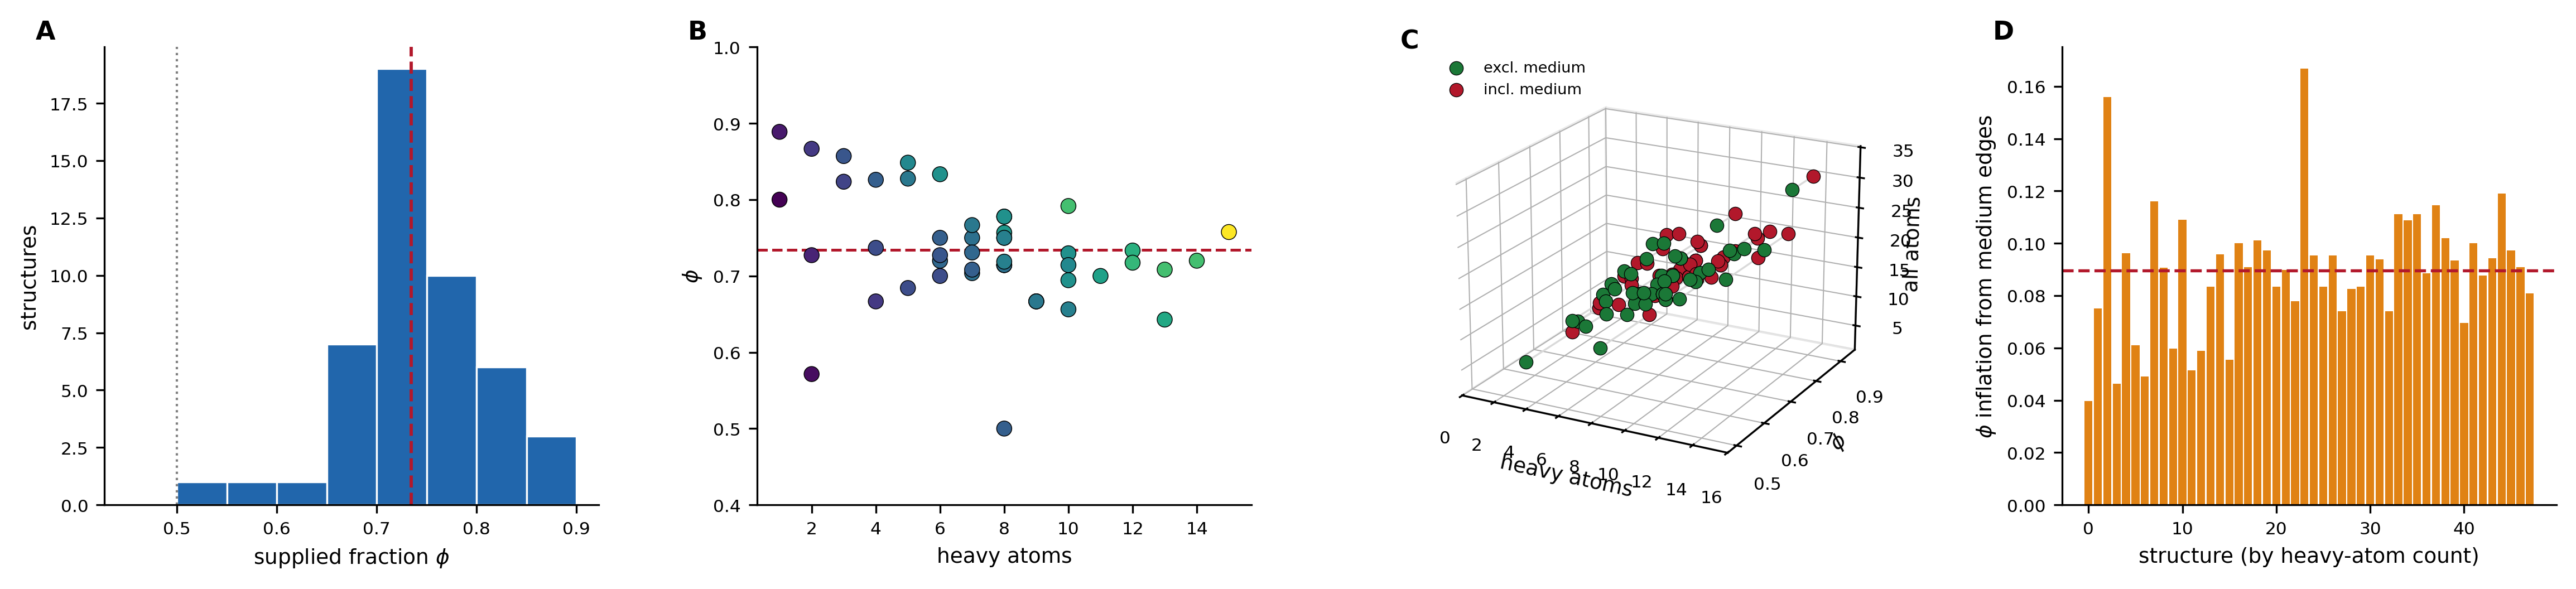
\includegraphics[width=\textwidth]{figures/panel_01_supplied.png}
    \caption{\textbf{Across a $48$-structure corpus a mean of $73.4\%$ of
    a SMILES-derived contact graph is supplied by convention rather than
    stated by the record, and no structure falls below $50.0\%$.}
    $\phi$ (\Cref{def:suppfrac}) ranges over the graph's own vertices and
    contacts; medium edges are excluded, for the reason defect D2 gives
    and panel~(\textbf{D}) measures.
    (\textbf{A})~Distribution of $\phi$, with the corpus mean $0.734$
    dashed and $0.500$ dotted. The distribution is tight --- standard
    deviation $0.071$ --- and lies entirely above $0.5$. We had expected
    the corpus to contain records stating everything the request needed,
    giving $\phi=0$ exactly; it contains none, which
    \Cref{rem:nozero} records as a fact about the format rather than
    about the reader.
    (\textbf{B})~$\phi$ against heavy-atom count, coloured by total atom
    count. The cloud is close to flat: the supplied fraction is a property
    of the notation's conventions rather than of molecular size, so it
    does not wash out as structures grow.
    (\textbf{C})~The corrected and uncorrected statistics for every
    structure, joined per structure. Green points exclude medium edges and
    red include them; the vertical segment is the inflation. The two point
    clouds never cross, so the correction changes the value of $\phi$
    everywhere without changing its ordering.
    (\textbf{D})~The inflation itself, one bar per structure ordered by
    heavy-atom count, with the mean $0.089$ dashed. It runs from $0.040$
    to $0.167$ and is largest on the smallest molecules --- because every
    medium edge is $\supplied$ by construction, including them makes
    $\phi$ a quantity dominated by the target representation exactly where
    the source record is shortest. That is defect D2 as a measurement
    rather than as an argument.}
    \label{fig:supplied}
\end{figure*}

\begin{figure*}[!htbp]
    \centering
    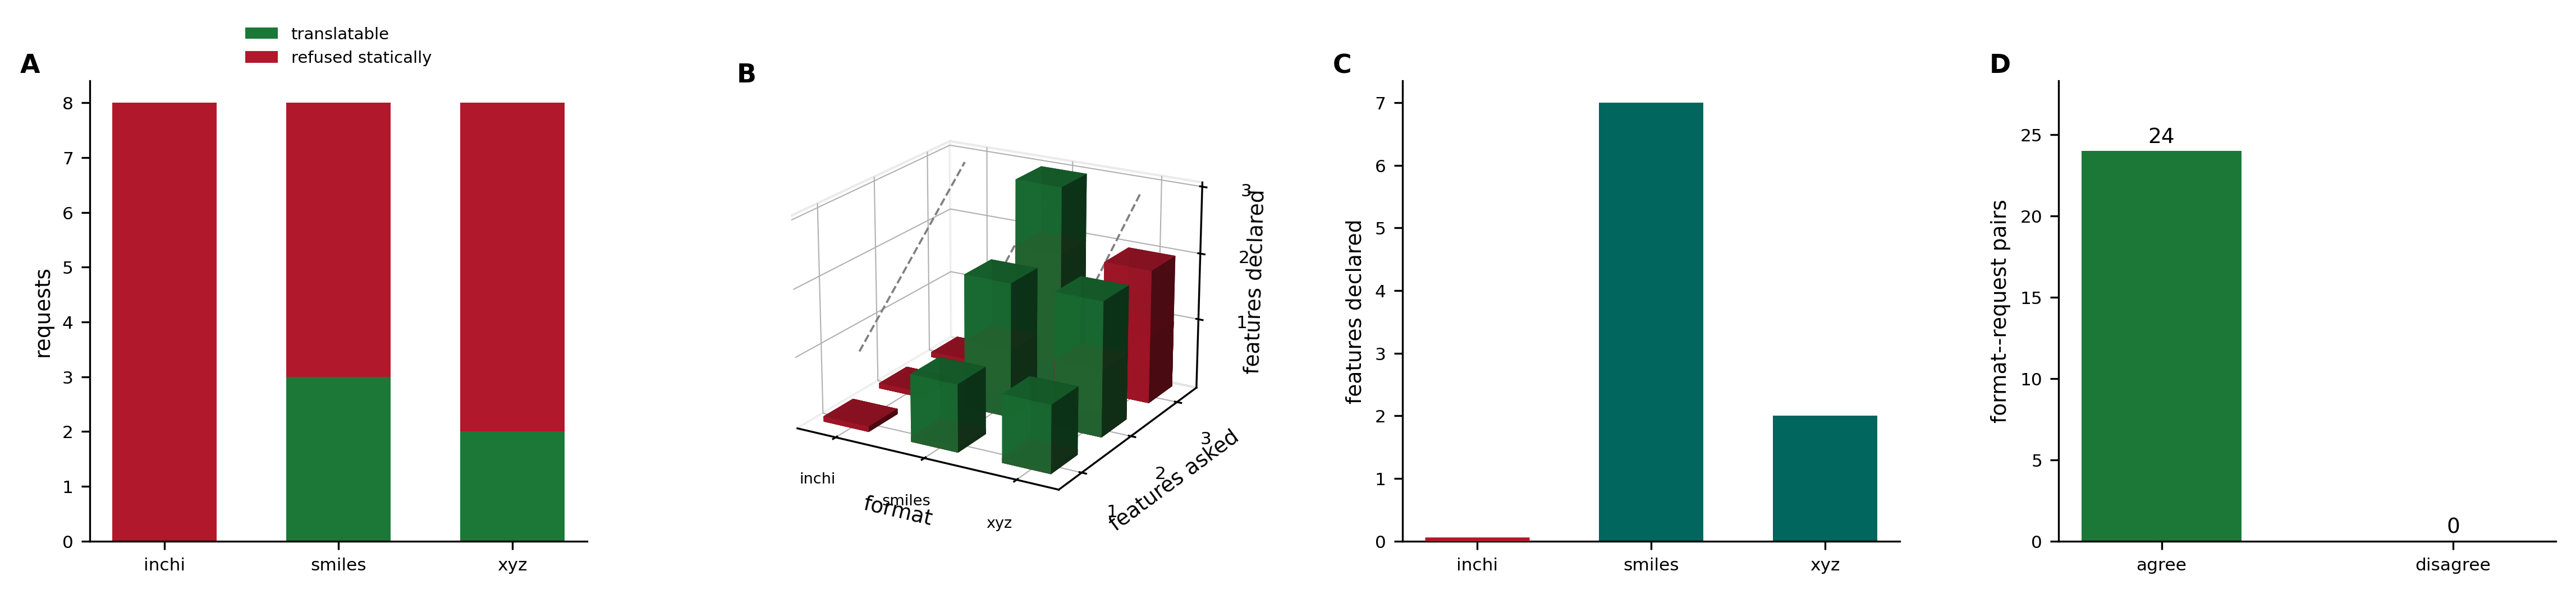
\includegraphics[width=\textwidth]{figures/panel_02_capability.png}
    \caption{\textbf{Capability containment decides $19$ of $24$
    format--request pairs before any record is read, and agrees with the
    post-read outcome on all $24$.}
    Each pair was checked twice: statically against the declared
    capability set (\Cref{cor:static}), and again by attempting the
    translation and inspecting the resulting label.
    (\textbf{A})~Requests per format, split into those refused statically
    and those a read may satisfy. The \textsf{inchi} row refuses all
    eight, because no reader is implemented and the capability set is
    empty --- an honest under-declaration, which \Cref{sec:capability}
    argues is the safe direction to err in.
    (\textbf{B})~Each pair as a bar over (format, features asked), with
    height the number of asked-for features the format actually declares
    and the dashed diagonal marking full service. A bar reaching the
    diagonal is translatable; one short of it is refused. Height is
    features \emph{declared} rather than features \emph{missing} because
    the latter renders every satisfiable request as a zero-height,
    invisible bar.
    (\textbf{C})~Declared capability size per format: seven features for
    SMILES, two for the coordinate-only reader, none for \textsf{inchi}.
    The zero is drawn as an explicit floor tick so that a format declaring
    nothing is legible as a measured zero rather than as an absent bar.
    (\textbf{D})~Agreement between the static verdict and the post-read
    outcome, over all $24$ pairs. The disagreement count is zero. The
    direction that would matter is a static refusal of a request a read
    would have satisfied, since that is the unsound one; there were
    none.}
    \label{fig:capability}
\end{figure*}

\begin{figure*}[!htbp]
    \centering
    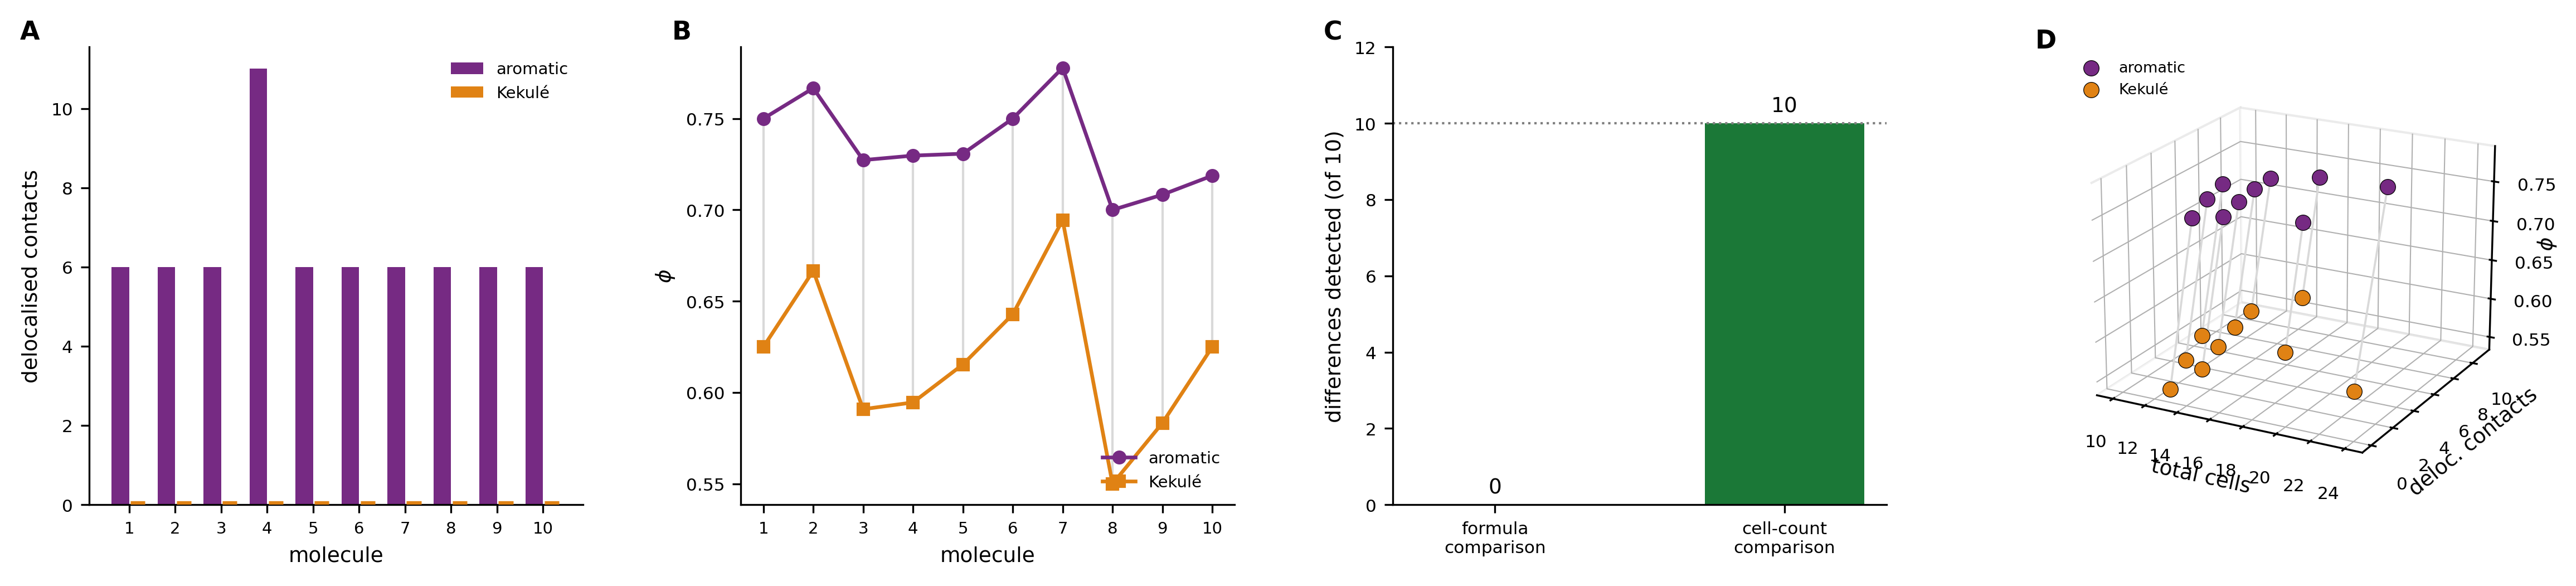
\includegraphics[width=\textwidth]{figures/panel_03_disagreement.png}
    \caption{\textbf{Ten molecules written two faithful ways yield ten
    pairs of contact graphs that differ, while formula-level comparison
    reports agreement on all ten.}
    Each molecule is expressed once with a lower-case aromatic ring and
    once in an alternating Kekul\'e assignment. Both translations state
    exactly what their source states, so neither is a misreading.
    (\textbf{A})~Delocalised contacts under each reading. The aromatic
    form yields six per benzenoid ring (eleven for naphthalene); the
    Kekul\'e form yields none, drawn as explicit floor ticks so the zeros
    read as measured rather than missing. By \Cref{prop:deloc} neither
    graph converts into the other without supplying a fact.
    (\textbf{B})~The supplied fraction under each reading, joined per
    molecule. The Kekul\'e form is lower in every case --- benzene gives
    $0.750$ against $0.625$ --- because stating per-contact cell counts
    removes them from what convention must supply. The gap is a
    measurement of how much the aromatic notation leaves to the reader.
    (\textbf{C})~What each comparison detects. A formula-level comparison
    finds $0$ of $10$ differences; a cell-count comparison finds $10$ of
    $10$. This is the paper's central practical claim in one measurement:
    the disagreement is real and the conventional instrument is blind to
    it, which is why \Cref{sec:disagreement} argues identity comparison is
    the wrong tool here.
    (\textbf{D})~The two readings in (total cells, delocalised contacts,
    $\phi$) space, joined per molecule. The two clouds are disjoint on
    every axis, and the connecting segments are all parallel: the
    disagreement is systematic, not sporadic. Note that the measured
    ratio is $10/10$ because these pairs were constructed to contain an
    aromatic ring; \Cref{rem:tenten} states that this measures visibility
    and not prevalence.}
    \label{fig:disagreement}
\end{figure*}

\begin{figure*}[!htbp]
    \centering
    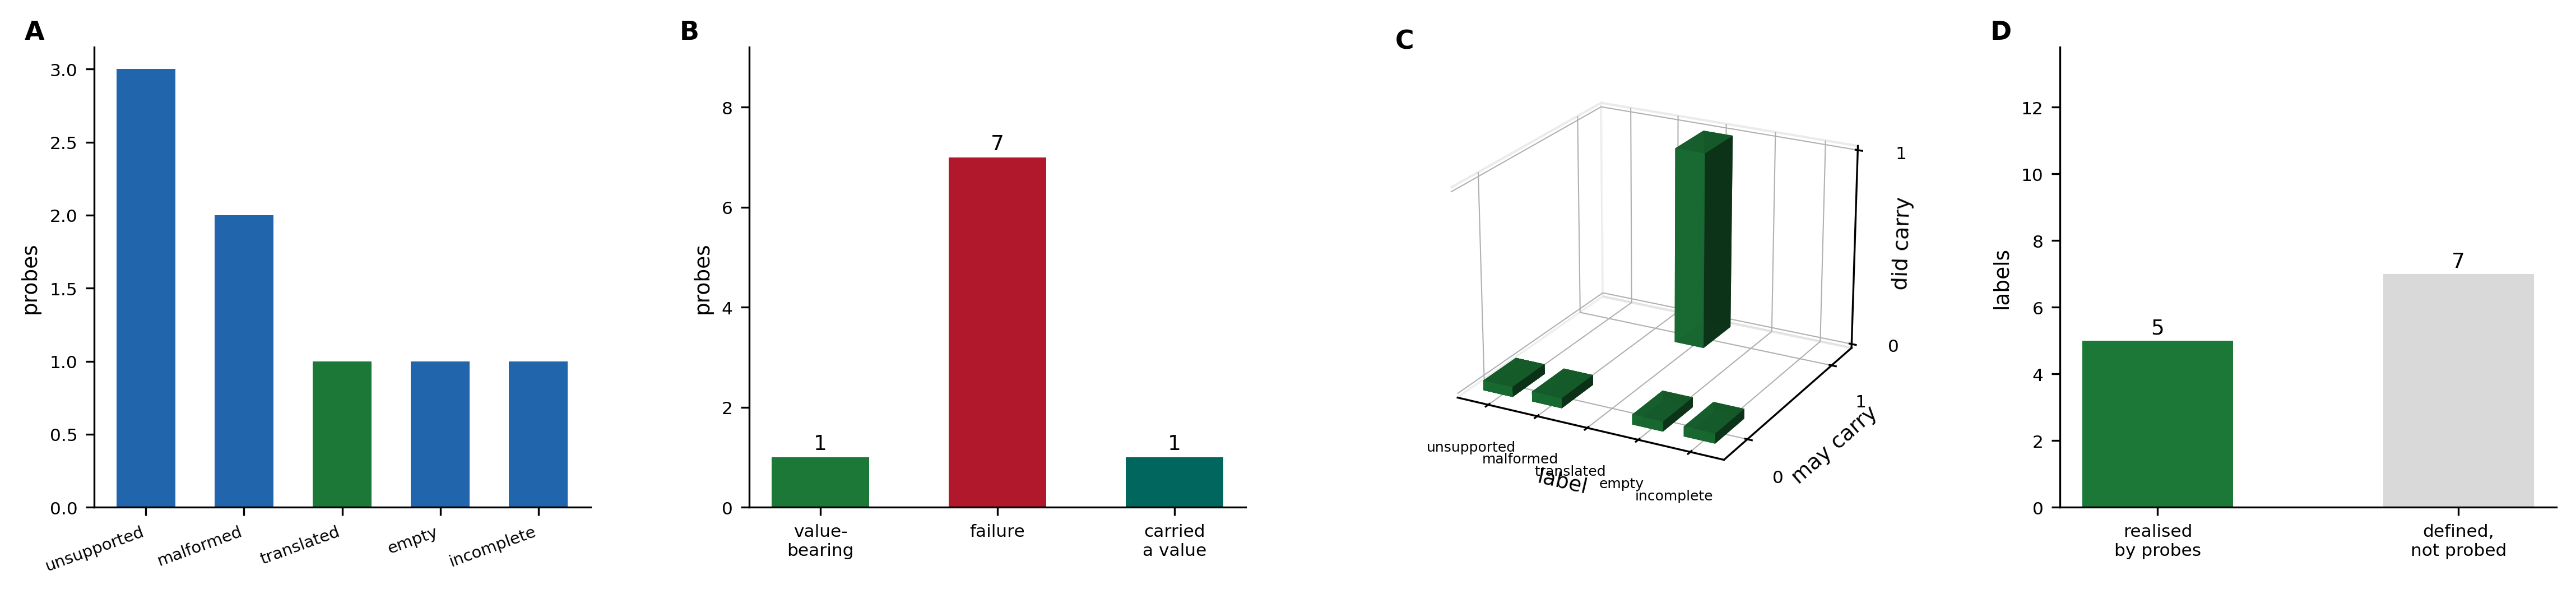
\includegraphics[width=\textwidth]{figures/panel_04_verdicts.png}
    \caption{\textbf{Eight probes realise five distinct verdict labels,
    and no failure verdict carries a value.}
    (\textbf{A})~Labels realised by the probe set. \textsf{empty} appears
    here only because of defect D4: the parser raised on empty input
    before clause (V2) was reached, so \textsf{empty} was unreachable from
    the SMILES path and an empty record was reported as
    \textsf{malformed}. That is the conflation \Cref{thm:conflation}
    identifies, occurring inside the implementation built to prevent it;
    \Cref{rem:d4} gives the account.
    (\textbf{B})~Probes by whether their label may carry a value, whether
    the label is a failure, and whether a value was in fact carried. One
    probe is value-bearing, seven are failures, and exactly one carried a
    value --- the same one. The failure column is the population in which
    a violation could occur, and it is empty.
    (\textbf{C})~Each probe positioned by label, by whether its label may
    carry a value, and by whether it did. Every bar sits at $\text{did
    carry}=0$ except the single \textsf{translated} probe, and no bar sits
    in the region (may carry $=0$, did carry $=1$) that would constitute a
    violation. That region is empty by construction as well as by
    measurement: the invariant is enforced in the verdict constructor, so
    this panel confirms the constructor is reached rather than
    establishing the property independently.
    (\textbf{D})~Labels realised by these probes against those defined but
    not probed. Five of twelve are exercised. The unexercised seven are
    plan-level and honjo-level labels outside the translation path, and we
    make no claim about them here.}
    \label{fig:verdicts}
\end{figure*}


% =====================================================================
\section{What Masamune does not do}
\label{sec:limits}
% =====================================================================

\begin{enumerate}[label=\textbf{L\arabic*.},leftmargin=2.8em,itemsep=4pt]

\item \textbf{Honest declaration is assumed, never verified.} The whole
of \Cref{thm:capability} and \Cref{prop:tight} rests on
\Cref{def:honest}. Under-declaration is safe; over-declaration is
unsound and silent, since the check passes and a graph is produced
asserting a feature the reader did not faithfully extract. We know of no
mechanical check short of differential testing against an independent
reader. This is the largest gap and we do not minimise it
(\Cref{rem:honesty}).

\item \textbf{The supplied fraction counts, it does not weigh.} $\phi$
treats every element alike, so a supplied bond order at a reactive
centre and a supplied aliphatic hydrogen contribute equally
(\Cref{rem:suppfrac-limits}). A weighted variant would require a model
of which elements matter for which purpose, which is chemistry outside
this specification.

\item \textbf{No adjudication between sources.} When two records of the
same compound yield different graphs (\Cref{sec:disagreement}), Masamune
reports both with their provenance and the locus of difference. It does
not decide. Deciding requires knowing which source is right, which is
not a property of the records.

\item \textbf{No repair.} A record that cannot be faithfully translated
yields a refusal, never a best-effort graph. This is deliberate and it
has a cost: pipelines that currently proceed on repaired structures will
instead halt, and the analyst must decide what to do. We regard
surfacing that decision as the point, but it is a cost.

\item \textbf{Conventions are declared, not validated.} A convention may
be documented, named, and wrong. Provenance records \emph{that} a
convention was applied and \emph{which}; it does not certify that the
convention is chemically sound.

\item \textbf{Contact weights are not specified here.} \Cref{def:contact}
requires $\wt>0$ but this paper fixes no particular weighting: what a
separation costs is a modelling decision belonging to whatever computes
on the graph. Every result above holds for any strictly positive
weighting, and none of them determines one.

\item \textbf{Coverage.} Readers are specified for line notations,
connection tables and coordinate records. Reaction formats, polymer and
Markush representations, and query languages such as SMARTS
\citep{daylight_smarts} are outside the present scope; the feature
alphabet of \Cref{def:features} would need extension, and
\Cref{prop:nameable-analogue} below states why that matters.
\end{enumerate}

\begin{proposition}[An unnameable feature is an undetectable omission]
\label{prop:nameable-analogue}
Let $f$ be a structural feature absent from $\Feat$. Then clause (V3) of
\Cref{def:assign} cannot fire on $f$, no verdict attributes any
discrepancy to $f$, and two readers differing only in whether they
extract $f$ produce graphs whose difference is unattributable.
\end{proposition}

\begin{proof}
(V3) is a containment test over $\Feat$; a symbol absent from $\Feat$
occurs in neither $\Req$ nor $\Capset(\Src)$, so the test cannot fire on
it. The remaining clauses do not mention features individually. Hence no
verdict names $f$, and a difference caused by $f$ is reported, if at
all, only as a difference between graphs with no attribution.
\end{proof}

\Cref{prop:nameable-analogue} is why \Cref{def:features} enumerates what
readers \emph{do} extract rather than only what requests commonly ask
for: the alphabet must be extended whenever a new structural feature
enters any reader, not only when a request needs it.

% =====================================================================
\section{Conclusion}
\label{sec:conclusion}
% =====================================================================

Chemical structure arrives in many formats, each stating some things and
silent about others, and the conventional conversion pipeline discards
the difference: after conversion, a supplied hydrogen and a recorded
hydrogen are the same object. We have specified a converter designed so
that this is not expressible.

The target is a contact graph (\Cref{def:contact}): atoms, contacts, and
an explicit medium vertex against which each atom is individuated, with
strictly positive separation costs so that every item has a well-posed
positive separation cost (\Cref{lem:positive}). The three disciplines
are provenance typing, which composes as a maximum over
$\stated<\supplied<\absent$ (\Cref{thm:prov-compose}) and so cannot be
laundered by round-tripping (\Cref{cor:roundtrip}); verdict-carrying
translation, of which only one label carries a graph
(\Cref{prop:one-graph}) and which the conventional graph-or-nothing
interface provably cannot represent (\Cref{thm:conflation}); and
declared capability, which makes a large class of translation failures
decidable before any file is opened (\Cref{cor:static}) and refuses
exactly the requests that could not have been served
(\Cref{prop:tight}).

The plan layer lifts these to corpus scale with a grammar, an
operational semantics, and determinism and provenance-monotonicity
theorems (\Cref{thm:plan-determinism,thm:prov-monotone}).

The measurements are the part we would most want a reader to carry away.
Over $48$ structures, a mean of $73.4\%$ of the elements of a
SMILES-derived contact graph are supplied by convention rather than
stated by the record, and no structure falls below $50.0\%$: we had
expected the corpus to contain records stating everything the request
needed, and it contains none. Capability containment refuses $19$ of
$24$ format--request pairs without reading anything and never refuses
one a read would have satisfied. And every one of ten molecules
expressed both as an aromatic ring and as an explicit Kekul\'e
assignment yields two graphs that differ while the molecular formula
agrees, because the distinction at issue---delocalisation against a
per-contact cell count---is one canonicalisation is designed to remove.
That last ratio is $10/10$ because the pairs were built to contain the
mechanism; it measures visibility, not prevalence.

What remains open is the assumption everything rests on. A capability
declaration is an assertion by whoever wrote the reader, and an
over-declaration is unsound and invisible. Whether it can be discharged
without differential testing against an independent implementation is
the question we would most like answered and the one we leave open.

\bibliographystyle{plainnat}
\bibliography{references}

\end{document}
